\chapter{File system}
\label{CH:FS}

The purpose of a file system is to organize and store data. File systems
typically support sharing of data among users and applications, as well as
\indextext{persistence}
so that data is still available after a reboot.

The xv6++ file system provides Unix-like files, directories, and pathnames
(see Chapter~\ref{CH:UNIX}), and stores its data on a virtio disk for
persistence. The file system addresses several challenges:
\begin{itemize}

\item The file system needs on-disk data structures to represent the tree
of named directories and files, to record the identities of the
blocks that hold each file's content, and to record which areas
of the disk are free.

\item The file system must support
\indextext{crash recovery}.
That is, if a crash (e.g., power failure) occurs, the file system must
still work correctly after a restart. The risk is that a crash might
interrupt a sequence of updates and leave inconsistent on-disk data
structures (e.g., a block that is both used in a file and marked free).

\item Different processes may operate on the file system at the same time,
so the file-system code must coordinate to maintain invariants.

\item Accessing a disk is orders of magnitude slower than accessing
memory, so the file system must maintain an in-memory cache of
popular blocks.

\end{itemize}

The rest of this chapter explains how xv6++ addresses these challenges.

%% 
%%  -------------------------------------------
%% 
\section{Overview}

The file system implementation is organized in layers, shown in
Figure~\ref{fig:fslayer}.
The disk layer reads and writes blocks on a virtio disk.
In xv6++ the disk is represented by \lstinline{kernel.disk}
(see \texttt{kernel/xv6pp.h}),
and the virtio driver is \lstinline{kernel.disk_driver}
(see \texttt{kernel/virtio\_driver.h}).
The buffer cache layer caches disk blocks and synchronizes access to them,
making sure that only one kernel thread at a time can modify the
data stored in any particular block. In xv6++ this is the
\lstinline{buffer_cache} class (see \texttt{kernel/buffer\_cache.h}).
The logging layer allows higher layers to wrap updates to several blocks in a
\indextext{transaction},
and ensures that the blocks are updated atomically in the
face of crashes (i.e., all of them are updated or none). In xv6++ this is
\lstinline{file_system_log} (see \texttt{kernel/file\_system\_log.h}).
The inode layer provides individual files, each represented as an
\indextext{inode}
with a unique i-number and some blocks holding the file's data.
In xv6++ inode management is implemented by \lstinline{file_system}
(see \texttt{kernel/file\_system.h}).
The directory layer implements each directory as a special kind of
inode whose content is a sequence of directory entries, each of which contains a
file's name and i-number.
The pathname layer provides hierarchical path names like
\lstinline{/usr/rtm/xv6/fs.c},
and resolves them with recursive lookup.
Finally, the file descriptor layer abstracts many Unix resources
(e.g., pipes, devices, files, etc.) using a uniform interface.

\begin{figure}[t]
\center
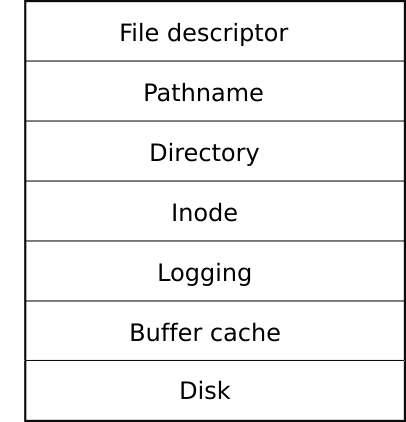
\includegraphics[scale=0.5]{fig/fslayer.pdf}
\caption{Layers of the xv6 file system.}
\label{fig:fslayer}
\end{figure}

Disk hardware traditionally presents the data on the disk as a numbered
sequence of 512-byte \textit{sectors}.
File systems typically use a larger block size, often a multiple of 512 bytes.
In xv6++ the file system block size is \lstinline{BSIZE} bytes
(see \texttt{kernel/fs.h}), and xv6++ reads and writes whole file-system
blocks through the buffer cache.

Xv6++ holds copies of disk blocks that it has read into memory
in objects of type \lstinline{struct buf}
(see \texttt{kernel/buffer\_cache.h}).
The data stored in a \lstinline{buf} can be temporarily out of sync with the disk:
it might not yet have been read in from disk, or it might have been updated by
software but not yet written back to disk.

The file system must have a plan for where it stores inodes and
content blocks on the disk. To do so, it divides the disk into several
sections, as Figure~\ref{fig:fslayout} shows.
The file system does not use
block 0 (it holds the boot sector). Block 1 is called the
\indextext{superblock};
it contains metadata about the file system (the file system size in blocks, the
number of data blocks, the number of inodes, and the number of blocks in the
log). Blocks starting at 2 hold the log. After the log are the inodes,
with multiple inodes per block. After those come bitmap blocks tracking which
data blocks are in use. The remaining blocks are data blocks; each is either
marked free in the bitmap block, or holds content for a file or directory.
The superblock is filled in by a separate program, \lstinline{mkfs}
(see \texttt{mkfs/mkfs.c}).

The rest of this chapter discusses each layer, starting with the
buffer cache. Look out for situations where well-chosen abstractions at lower
layers ease the design of higher ones.

\begin{figure}[t]
\center
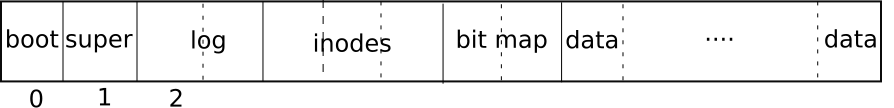
\includegraphics[scale=0.5]{fig/fslayout.pdf}
\caption{Structure of the xv6 file system.}
\label{fig:fslayout}
\end{figure}

%% 
%%  -------------------------------------------
%% 
\section{Buffer cache layer}
\label{s:bcache}

The buffer cache has two jobs:
(1) synchronize access to disk blocks to ensure that only one copy of a block
is in memory and that only one kernel thread at a time uses that copy;
(2) cache popular blocks so that they don't need to be re-read from
the slow disk.

In xv6++ the buffer cache is implemented by \lstinline{class buffer_cache}
(see \texttt{kernel/buffer\_cache.h} and \texttt{kernel/buffer\_cache.cpp}).
Its primary interface is:

\begin{itemize}
\item \lstinline{buf* buffer_cache::read(uint dev, uint blockno)}
\item \lstinline{void buffer_cache::write(buf* b)}
\item \lstinline{void buffer_cache::relse(buf* b)}
\item \lstinline{void buffer_cache::pin(buf* b)} and \lstinline{unpin(buf* b)}
\end{itemize}

A kernel thread obtains a \lstinline{buf} with \lstinline{read()},
uses the buffer while holding the buffer's sleep-lock, and then releases it
with \lstinline{relse()} when finished.
The buffer cache uses a per-buffer sleep-lock so that only one thread at a time
uses each buffer (and thus each disk block).

Xv6++ also provides an optional RAII helper, \lstinline{buffer_guard}
(see \texttt{kernel/buffer\_guard.h}),
which automatically releases a buffer when the guard object goes out of scope:

\begin{lstlisting}
{
  buffer_guard bg(dev, blockno);
  // use bg->data[] while locked
} // automatically calls kernel.cache.relse(...)
\end{lstlisting}

The buffer cache has a fixed number of buffers to hold disk blocks.
If the file system asks for a block that is not already in the cache,
the buffer cache must recycle a buffer currently holding some other block.
The buffer cache recycles the least recently used buffer for the new block.
The assumption is that the least recently used buffer is the one least likely
to be used again soon.

%% 
%%  -------------------------------------------
%% 
\section{Code: Buffer cache}

The buffer cache contains a fixed \lstinline{storage[NBUF]} array of buffers,
and maintains an LRU list using an intrusive doubly-linked list
(see \texttt{kernel/intrusive\_dlist.h}).
The cache metadata is protected by a spinlock, while each individual buffer
is protected by its own sleep-lock.

\lstinline{buffer_cache::read(dev, blockno)} obtains a locked buffer for the
given device and block number. If the buffer is not yet valid, the cache asks
the disk driver to fill it by initiating a read through the block device.
In xv6++ the virtio driver methods operate on \lstinline{buf*} objects and are
invoked through the disk abstraction (see \texttt{kernel/block\_device.h} and
\texttt{kernel/virtio\_driver.h}).

The cache must ensure that there is at most one cached buffer per disk block.
This invariant ensures that readers see writes, and it is also fundamental to
synchronization: higher layers rely on buffer locks to serialize updates to
important blocks such as the free-space bitmap.
Xv6++ enforces this invariant by holding the buffer cache spinlock across the
steps of checking for an existing buffer and, if necessary, selecting and
installing a buffer for the requested block.

If all buffers are busy, then too many processes are simultaneously executing
file system calls; the cache panics. A more graceful response might be to sleep
until a buffer became free, though there would then be a possibility of deadlock.

When the caller is done with a buffer it calls \lstinline{relse()}.
The release operation moves the buffer to the most-recently-used end of the LRU
list, implementing an LRU replacement policy.

%% 
%%  -------------------------------------------
%% 
\section{Logging layer}

One of the most interesting problems in file system design is crash recovery.
The problem arises because many file-system operations involve multiple writes
to the disk, and a crash after a subset of the writes may leave the on-disk file
system in an inconsistent state. For example, suppose a crash occurs during file
truncation (setting the length of a file to zero and freeing its content blocks).
Depending on the order of disk writes, the crash may either leave an inode with a
reference to a content block that is marked free, or it may leave an allocated but
unreferenced content block.

The latter is relatively benign, but an inode that refers to a freed block is
likely to cause serious problems after a reboot. After reboot, the kernel might
allocate that block to another file, and now we have two different files pointing
unintentionally to the same block.

Xv6++ solves the problem of crashes during file-system operations with a simple
form of write-ahead logging. A system call does not directly write the on-disk file
system data structures. Instead, it records the blocks it wishes to modify in a
\indextext{log} on disk. Once the system call has logged all of its writes, it
writes a special \indextext{commit} record indicating that the log contains a
complete operation. At that point the system call copies the writes to their home
locations in the on-disk file system. After those writes complete, the system call
erases the log on disk.

If the system crashes and reboots, the file-system code recovers from the crash
before running any processes. If the log is marked as containing a complete
operation, the recovery code copies the writes to where they belong in the on-disk
file system. If the log is not marked complete, the recovery code ignores it. The
recovery code finishes by erasing the log.

Why does this solve crash consistency? If the crash occurs before commit, then the
log will not be marked complete and recovery ignores it, leaving the disk as if the
operation never started. If the crash occurs after commit, recovery will replay the
log, ensuring that all of the operation’s updates appear on disk. Thus operations
are atomic with respect to crashes: after recovery, either all updates appear, or
none do.

%% 
%% 
%% 
\section{Log design}

The log resides at a known fixed location, specified in the superblock.
It consists of a header block followed by a sequence of updated block copies
(“logged blocks”). The header block contains an array of block numbers, one for
each logged block, and the count of logged blocks.

The count in the header block on disk is either zero, indicating that there is no
transaction in the log, or non-zero, indicating that the log contains a complete
committed transaction with the indicated number of logged blocks. The log writes
the header block when a transaction commits, but not before, and sets the count
to zero after copying logged blocks to their home locations.

Each system call indicates the start and end of the sequence of writes that must be
atomic with respect to crashes. To allow concurrent execution of file-system
operations by different processes, the logging system can accumulate the writes of
multiple system calls into one transaction. Thus a single commit may include the
writes of multiple complete system calls. To avoid splitting a system call across
transactions, the logging system only commits when no file-system system calls are
underway.

Committing several operations together is known as
\indextext{group commit}.
Group commit reduces disk operations by amortizing the fixed cost of a commit over
multiple operations.

Xv6++ dedicates a fixed amount of space on the disk to hold the log. The total
number of blocks written by the system calls in a transaction must fit in that
space. This implies:
(1) no single system call can be allowed to write more distinct blocks than the log
space allows; (2) a system call cannot begin unless the log can reserve enough space
for the call’s worst-case block writes.

%% 
%% 
%% 
\section{Code: logging}

In xv6++ the logging layer is implemented by \lstinline{class file_system_log}
(see \texttt{kernel/file\_system\_log.h} and \texttt{kernel/file\_system\_log.cpp})
and is available as \lstinline{kernel.log}.

A typical use looks like:

\begin{lstlisting}
  kernel.log.begin_op();
  ...
  buf *bp = kernel.cache.read(dev, blockno);
  bp->data[...] = ...;
  kernel.log.log_write(bp);
  kernel.cache.relse(bp);
  ...
  kernel.log.end_op();
\end{lstlisting}

\lstinline{begin_op()} waits until the logging system is not currently committing,
and until there is enough unreserved log space to hold the writes from this call.
The log conservatively assumes that each file-system system call might write up to
\lstinline{MAXOPBLOCKS} distinct blocks (see \texttt{kernel/param.h}).

\lstinline{log_write(bp)} acts as a proxy for writing a dirty buffer to disk. It
records the block number in memory, reserving it a slot in the on-disk log, and pins
the buffer in the cache so that it cannot be evicted until commit completes.
The cached copy is the only record of the modification until commit installs the
transaction.

If a block is written multiple times during a single transaction, \lstinline{log_write}
assigns it a single slot in the log. This optimization is called
\indextext{absorption}.

\lstinline{end_op()} decrements the count of outstanding operations. If the count drops
to zero, it commits the current transaction. The commit process has four conceptual stages:

\begin{itemize}
\item Copy modified blocks from the cache to their slots in the on-disk log.
\item Write the log header block: this is the commit point.
\item Install (copy) logged blocks to their home locations in the file system.
\item Clear the log header (count zero), erasing the transaction.
\end{itemize}

Recovery runs during boot, before the first user process executes. The recovery code
reads the log header and, if it indicates a committed transaction, installs the logged
blocks to their home locations and then clears the log.

%% 
%% 
%% 
\section{Code: Block allocator}

File and directory content is stored in disk blocks, which must be allocated from a free pool.
The block allocator maintains a free bitmap on disk, with one bit per block.
A zero bit indicates that the corresponding block is free; a one bit indicates that it is in use.
The program \lstinline{mkfs} sets the bits corresponding to the boot sector, superblock, log blocks,
inode blocks, and bitmap blocks.

The block allocator provides two functions:
\lstinline{balloc} allocates a new disk block, and \lstinline{bfree} frees a block.
In xv6++ these are methods on \lstinline{file_system}
(see \texttt{kernel/file\_system.h} and \texttt{kernel/file\_system.cpp}).

The allocator scans bitmap blocks looking for a free bit. The race that might occur if two
processes try to allocate a block at the same time is prevented by the fact that the buffer
cache only allows one thread at a time to hold the bitmap block buffer lock.

As with much of the code described in this chapter, \lstinline{balloc} and \lstinline{bfree}
must be called inside a transaction.

%% 
%%  -------------------------------------------
%% 
\section{Inode layer}

The term \indextext{inode} can refer to either:
(1) the on-disk inode data structure, which contains a file’s size and list of block numbers; or
(2) an in-memory inode, which caches the on-disk inode and includes kernel-only state.

The on-disk inode is defined by \lstinline{struct dinode} (see \texttt{kernel/fs.h}).
The in-memory inode is defined by \lstinline{struct inode} (see \texttt{kernel/file\_system.h}).

The on-disk inode fields include:
\lstinline{type} (file vs directory vs device),
\lstinline{nlink} (number of directory entries referencing the inode),
\lstinline{size} (file size in bytes),
and \lstinline{addrs[]} (disk block addresses).

The kernel keeps a fixed-size cache of active in-memory inodes.
In xv6++ that cache lives inside \lstinline{class file_system} as
\lstinline{inode inodes[NINODE]} protected by a spinlock.

There are several lock or lock-like mechanisms associated with inodes:
a global inode-table lock protects the inode table invariants and reference counts;
each inode has a sleep-lock to provide exclusive access to the inode’s metadata and content;
the reference count prevents reuse of an in-memory inode entry while it is referenced;
and the on-disk link count prevents freeing an inode that is still reachable from a directory.

A pointer to an inode returned by \lstinline{iget()} is valid until the corresponding \lstinline{iput()}:
the inode will not be deleted and the memory for that inode will not be reused.

\lstinline{iget()} provides non-exclusive access so that there may be multiple pointers to the same inode.
To read or modify an inode’s metadata or file content, code must lock it with \lstinline{ilock()},
which also ensures that the inode has been read from disk. \lstinline{iunlock()} releases the inode lock.

Separating acquisition of inode pointers from inode locking helps avoid deadlock in pathname resolution.

%% 
%%  -------------------------------------------
%% 
\section{Code: Inodes}

To allocate a new inode (for example, when creating a file), xv6++ calls
\lstinline{file_system::ialloc()}.
This scans on-disk inode blocks looking for a free inode (type zero), claims it,
writes the new type to disk, and returns the corresponding in-memory inode.

\lstinline{iget()} looks in the in-memory inode cache for an existing entry with matching device and inode number.
If it finds one, it increments the reference count and returns it. Otherwise it allocates a free cache entry.

\lstinline{ilock()} acquires the inode’s sleep-lock. If the inode has not yet been read from disk,
\lstinline{ilock()} reads the on-disk inode into the in-memory inode structure.

\lstinline{iput()} decrements the reference count. If it drops to zero and the on-disk link count is also zero,
the inode and its data blocks must be freed. That process truncates the file, clears the inode type on disk,
and updates the inode on disk.

Even read-only system calls may call \lstinline{iput()} on their way out, and \lstinline{iput()} can write to disk.
For that reason, system calls that use the file system must be prepared to participate in logging transactions.

Xv6++ retains the same basic design as xv6 here: it does not implement a full orphan-inode recovery mechanism,
so a crash can leave allocated but unlinked inodes on disk.

%% 
%% 
%% 
\section{Code: Inode content}

\begin{figure}[t]
\center
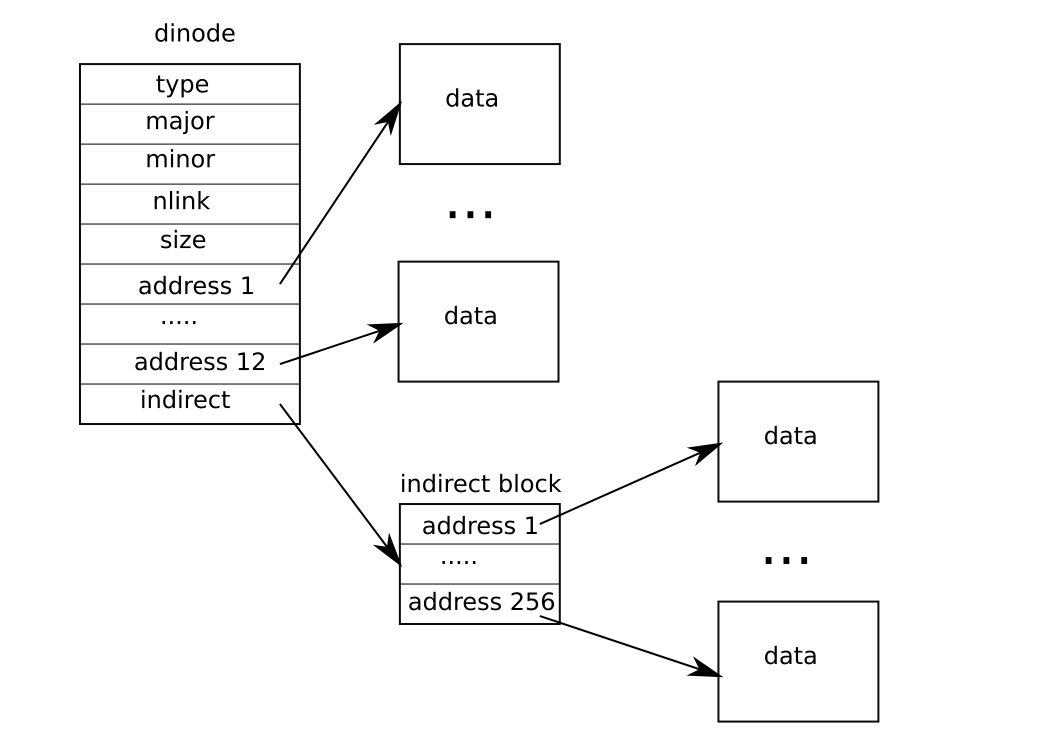
\includegraphics[scale=0.5]{fig/inode.pdf}
\caption{The representation of a file on disk.}
\label{fig:inode}
\end{figure}

The on-disk inode structure \lstinline{struct dinode} contains a file size and an array of block numbers
(see Figure~\ref{fig:inode}). The first \lstinline{NDIRECT} blocks are \indextext{direct blocks}
whose addresses are stored directly in \lstinline{addrs[]}.
The final pointer in \lstinline{addrs[]} refers to the \indextext{indirect block}, which contains a further
array of block addresses.

This representation is efficient on disk but somewhat complex for clients. The method \lstinline{bmap()}
hides the details: it maps a file’s logical block number to a disk block number, allocating blocks as needed.

Truncation frees all of a file’s blocks and resets its size to zero; this is implemented by \lstinline{itrunc()}.

The methods \lstinline{readi()} and \lstinline{writei()} implement reading and writing bytes of a file by
iterating over file blocks, using \lstinline{bmap()} to locate each block, and copying bytes between user memory
and buffer-cache blocks.

\lstinline{stati()} copies inode metadata into a \lstinline{struct stat} exposed to user space by the \lstinline{stat} system call.

%% 
%% 
%% 
\section{Code: directory layer}

A directory is implemented internally much like a file. Its inode has type \lstinline{T_DIR}
and its data is a sequence of \lstinline{struct dirent} entries (see \texttt{kernel/fs.h}),
each containing a name and inode number.

\lstinline{dirlookup()} searches a directory for an entry with the given name. If it finds one,
it returns a pointer to the corresponding inode (obtained via \lstinline{iget()}), typically unlocked,
so that pathname traversal can avoid deadlock scenarios involving \lstinline{.} and \lstinline{..}.

\lstinline{dirlink()} creates a new directory entry. It scans the directory for a free slot (inode number zero),
or appends a new slot at the end, then writes the directory entry.

%% 
%% 
%% 
\section{Code: Path names}

Pathname lookup involves a sequence of \lstinline{dirlookup()} calls, one per path component.
\lstinline{namei()} returns the inode for a pathname.
\lstinline{nameiparent()} is a variant that stops one element early and returns the parent directory inode,
copying the final element into a caller-provided buffer.

Both rely on a helper that repeatedly locks the current directory inode, checks that it is a directory,
looks up the next path element, and then unlocks the current inode before locking the next.
This discipline avoids deadlocks such as trying to lock the same inode twice when traversing \lstinline{"."}.

Xv6++ is designed so that two independent pathname lookups can proceed concurrently as long as they operate
in different directories. Each directory inode has its own lock, and the buffer cache allows concurrent access
to different blocks.

%% 
%% 
%% 
\section{File descriptor layer}

A cool aspect of the Unix interface is that most resources are represented as files, including devices such as
the console, pipes, and real disk files. The file descriptor layer provides this uniformity.

Each process contains a per-process table of open file pointers,
\lstinline{file* ofile[NOFILE]} (see \texttt{kernel/process.h}).
Each open file is represented by \lstinline{class file} (see \texttt{kernel/file.h}),
which wraps either an inode or a pipe, plus an I/O offset.
Multiple processes can share the same open file object via \lstinline{fork()} or \lstinline{dup()}.

All open file objects are allocated from a global table managed by \lstinline{file_manager}
(see \texttt{kernel/file\_manager.h} and \texttt{kernel/file\_manager.cpp}).
\lstinline{file_manager} allocates and tracks \lstinline{file} objects and pipe objects.

The \lstinline{file} methods \lstinline{read()}, \lstinline{write()}, and \lstinline{stat()}
dispatch either to pipe code or inode code, depending on the file type.
Inodes use the per-file offset, and inode locking ensures that offset updates are atomic when multiple
writers share an open file.

%% 
%% 
%% 
\section{Code: System calls}

File-related system calls are implemented in \texttt{kernel/sysfile.cpp}.
Most are straightforward wrappers that:
(1) fetch user arguments,
(2) locate or create inodes and files,
(3) perform file operations,
(4) update reference counts and return results.

Some system calls must update multiple disk structures and therefore execute within a transaction,
using \lstinline{kernel.log.begin_op()} and \lstinline{kernel.log.end_op()}.
For example, creating and linking directory entries, allocating inodes and blocks, and updating bitmaps
must be crash-safe.

\lstinline{open} may create a file, which requires allocating an inode, initializing it, and linking it
into its parent directory. \lstinline{link} adds a new directory entry and increments the inode’s link count.
\lstinline{unlink} removes a directory entry and decrements the inode’s link count; if it drops to zero and
no file descriptors reference it, the inode and its blocks will be freed.

\lstinline{sys_pipe} allocates a pipe and installs two file descriptors referring to its read and write ends,
connecting the pipe implementation (Chapter~\ref{CH:SLEEP}) to the file interface.

%% 
%%  -------------------------------------------
%% 
\section{Real world}

The buffer cache in a real-world operating system is significantly more complex than xv6++'s, but it serves the
same two purposes: caching and synchronizing access to the disk.
Xv6++ uses a simple LRU eviction policy; many more complex policies exist.

Xv6++'s logging system is also intentionally simple.
A commit cannot occur concurrently with file-system system calls.
The system logs entire blocks, even if only a few bytes change.
Real systems address these issues with more sophisticated logging, delayed writes, and finer-grained metadata logging.

Logging is not the only way to provide crash recovery. Older file systems used a scavenger during reboot
(such as \lstinline{fsck}) to examine the disk and repair inconsistencies.
Logging speeds recovery and preserves atomicity for system calls.

Modern file systems often use different on-disk structures than early Unix designs:
directories implemented as trees, extent-based allocation, copy-on-write block trees,
snapshots, and incremental backup.

Modern Unix systems also allow many resources to be accessed through the file interface:
named pipes, sockets, remotely-mounted file systems, and virtual file systems such as \lstinline{/proc}.
In many systems, open files carry a table of operation function pointers rather than \lstinline{if} statements.

%% 
%%  -------------------------------------------
%% 
\section{Exercises}

\begin{enumerate}

\item Why panic in \lstinline{balloc}? Can xv6++ recover?

\item Why panic in \lstinline{ialloc}? Can xv6++ recover?

\item Why doesn't \lstinline{file_manager} panic when it runs out of files?
Why is this more common and therefore worth handling?

\item Suppose the file corresponding to an inode gets unlinked by another process
between incrementing \lstinline{nlink} and creating a directory entry. Will the link be created correctly?
Why or why not?

\item Implement \lstinline{lseek}. Supporting \lstinline{lseek} will also require modifying file write behavior
to fill holes with zeros when seeking beyond end-of-file.

\item Add \lstinline{O_TRUNC} and \lstinline{O_APPEND} to \lstinline{open}, so that \lstinline{>} and \lstinline{>>}
operators work in the shell.

\item Modify the file system to support symbolic links.

\item Modify the file system to support named pipes.

\item Modify the file system and VM system to support memory-mapped files.

\end{enumerate}
